\section{SIMON}

\begin{frame}{SIMON 2n/mn \footfullcite{SimonSpeck}}
\begin{figure}[h!]
    \centering
    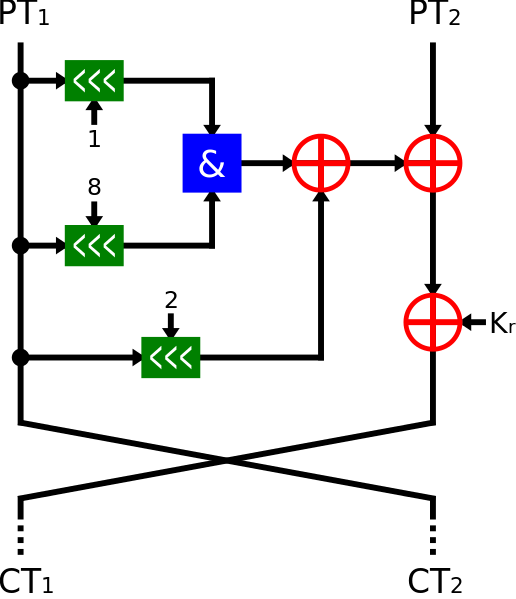
\includegraphics[width=0.3\linewidth]{simon/simon.png}
    \caption{One round of SIMON \cite{wiki:simon}}
    \label{fig:ors}
\end{figure}
\pause
\begin{block}{Round Function}
\begin{equation}\label{eq:simonfun}
    F(x,y) = (y\oplus (S^1(x)\wedge S^8(x)) \oplus S^2(x) \oplus k, x)
\end{equation}
\end{block}
\pause
\begin{itemize}
    \item $S^j(x)$ denotes left circular shift by j bits.
    \pause
    \item $PT_1, PT_2$ are also referred as $L_i, R_i$.
    \pause
    \item $CT_1, CT_2$ are also referred as $L_{i+1}, R_{i+1}$. $L_i, R_i$ are $n$ bit strings as input to the $i^{th}$ round and $k$ is the round key.
\end{itemize}
\end{frame}
\begin{frame}{Key Expansion}
    \begin{itemize}
        \item For the first $m$ rounds, the round keys are initialized from the master key.
        \pause
        \item For the remaining T-m rounds, use the below function:
    \end{itemize}
    \begin{equation}
 k_{m+i} = 
 \begin{cases} 
      c_i \oplus k_i \oplus S^{-3}(k_{i+1}) \oplus S^{-4}(k_{i+1}) &  m = 2 \\
      c_i \oplus k_i \oplus S^{-3}(k_{i+2}) \oplus S^{-4}(k_{i+2}) &  m = 3 \\
      c_i \oplus k_i \oplus S^{-1}(k_{i+1}) \oplus S^{-3}(k_{i+3}) \oplus S^{-4}(k_{i+3}) &  m = 4
  \end{cases}
\end{equation}
$c_i$ denotes the round constants.
\end{frame}